% Created 2017-11-17 Fri 08:16
% Intended LaTeX compiler: pdflatex
\documentclass[titlepage]{article}
\usepackage[utf8]{inputenc}
\usepackage[T1]{fontenc}
\usepackage{graphicx}
\usepackage{grffile}
\usepackage{longtable}
\usepackage{wrapfig}
\usepackage{rotating}
\usepackage[normalem]{ulem}
\usepackage{amsmath}
\usepackage{textcomp}
\usepackage{amssymb}
\usepackage{capt-of}
\usepackage{hyperref}
\hypersetup{hidelinks=true}
\setlength{\parindent}{2em}
\usepackage[margin=1in]{geometry}
\usepackage{indentfirst}
\author{Hu Xiaoxiang \\
U1521319A \\
EEE \\
}
\date{13 Nov, 2017 \\
}
\title{
\includegraphics[width=\textwidth]{logo_ntu_new.png} \\
[5\baselineskip] EE4483 \\
DATA-MINING ASSIGNMENT \\
REPORT \\
[5\baselineskip]}
\hypersetup{
 pdfauthor={Hu Xiaoxiang \\
U1521319A \\
EEE \\
},
 pdftitle={
\includegraphics[width=\textwidth]{logo_ntu_new.png} \\
[5\baselineskip] EE4483 \\
DATA-MINING ASSIGNMENT \\
REPORT \\
[5\baselineskip]},
 pdfkeywords={},
 pdfsubject={},
 pdfcreator={Emacs 25.1.1 (Org mode 9.1.2)}, 
 pdflang={English}}
\begin{document}

\maketitle
\tableofcontents

\pagenumbering{roman}
\newpage
\pagenumbering{arabic}

\section{Question 1:}
\label{sec:orga422168}
\begin{center}
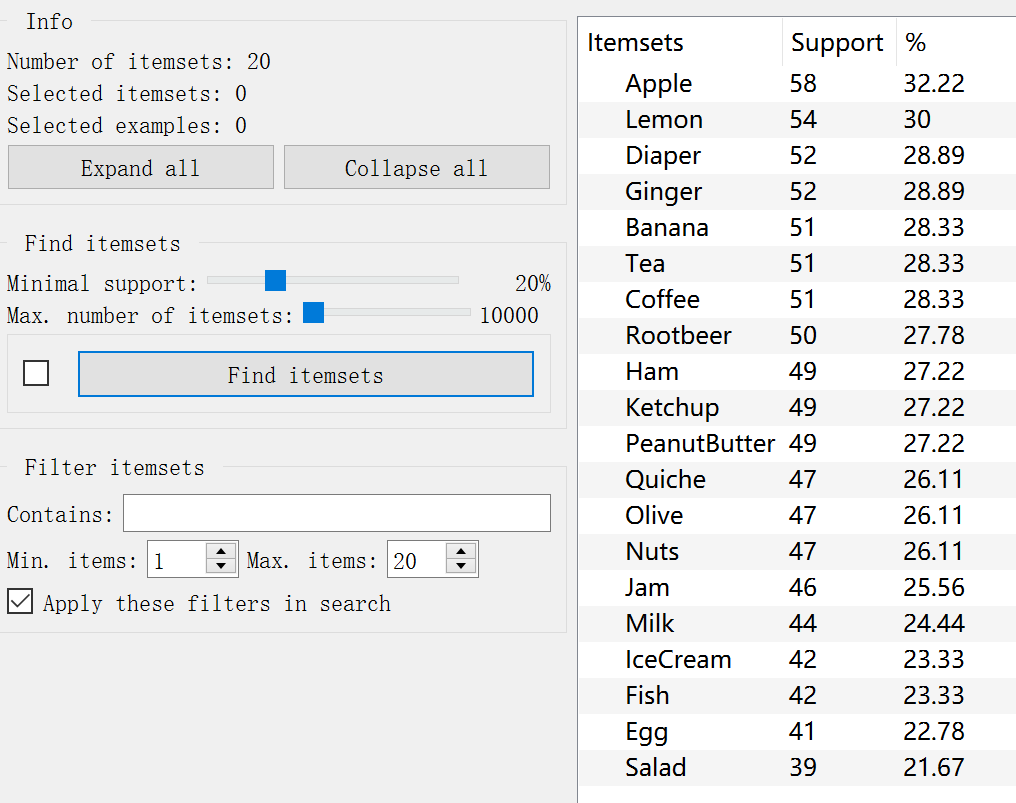
\includegraphics[width=0.49\textwidth]{minsup20.PNG}
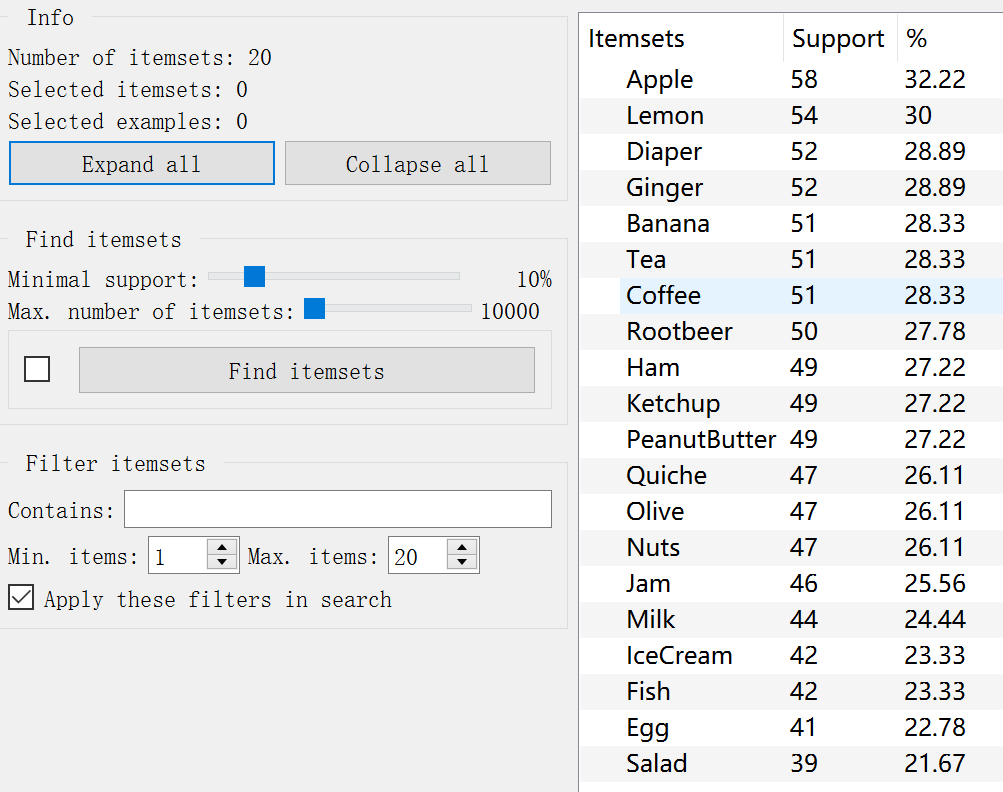
\includegraphics[width=0.49\textwidth]{minsup10.PNG}
\end{center}

\begin{center}
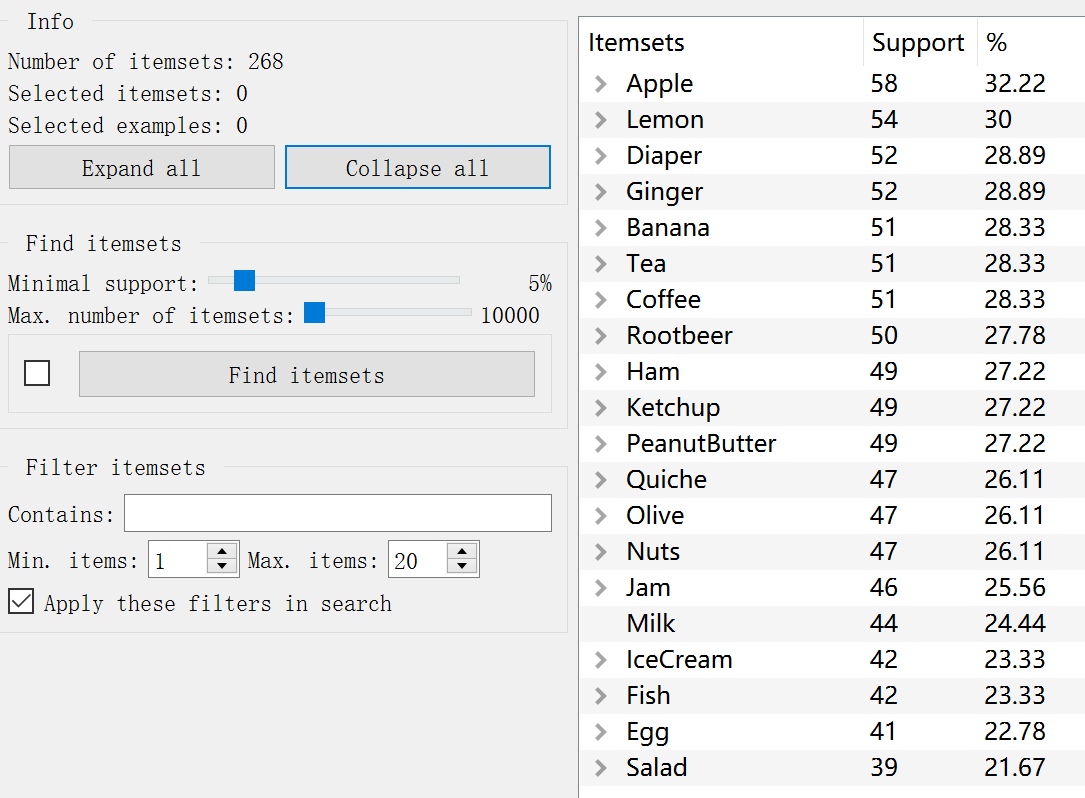
\includegraphics[width=0.49\textwidth]{minsup5.PNG}
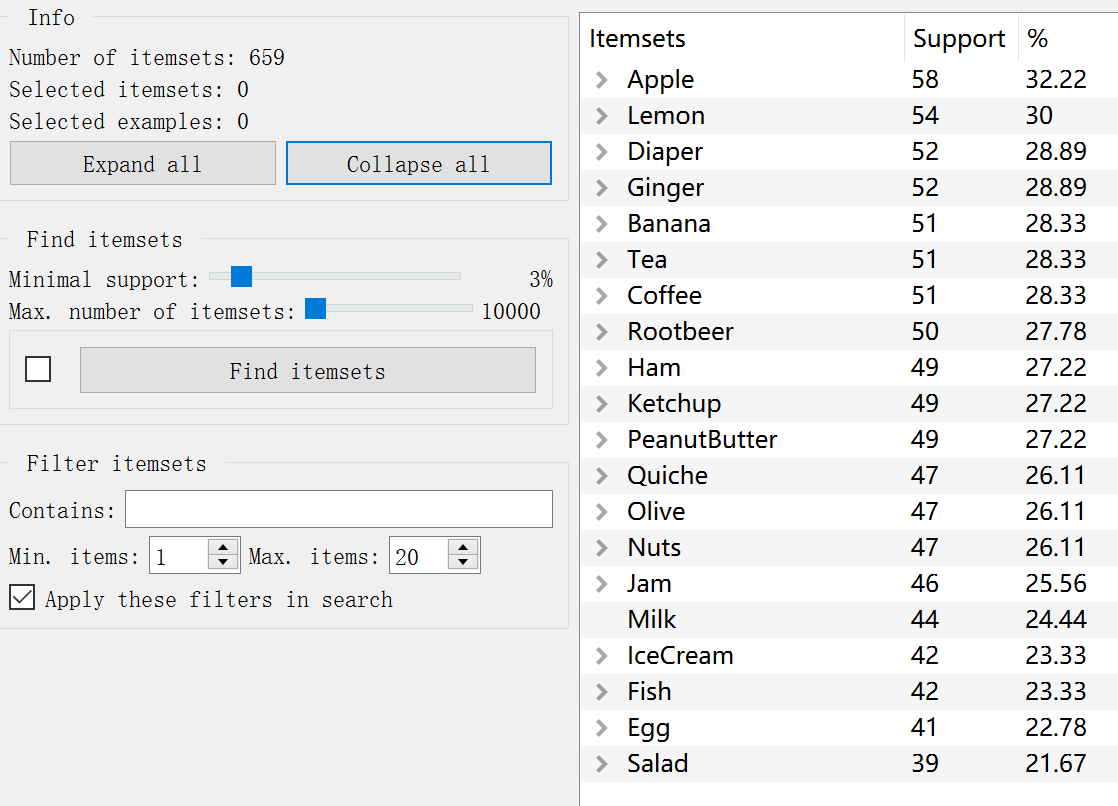
\includegraphics[width=0.49\textwidth]{minsup3.PNG}
\end{center}

\begin{center}
\begin{tabular}{rr}
\hline
Minimum Support (\%) & No. of Frequent Itemsets\\
20 & 20\\
10 & 68\\
5 & 268\\
3 & 659\\
\hline
\end{tabular}
\end{center}

\section{Question 2:}
\label{sec:orga826084}
\begin{center}
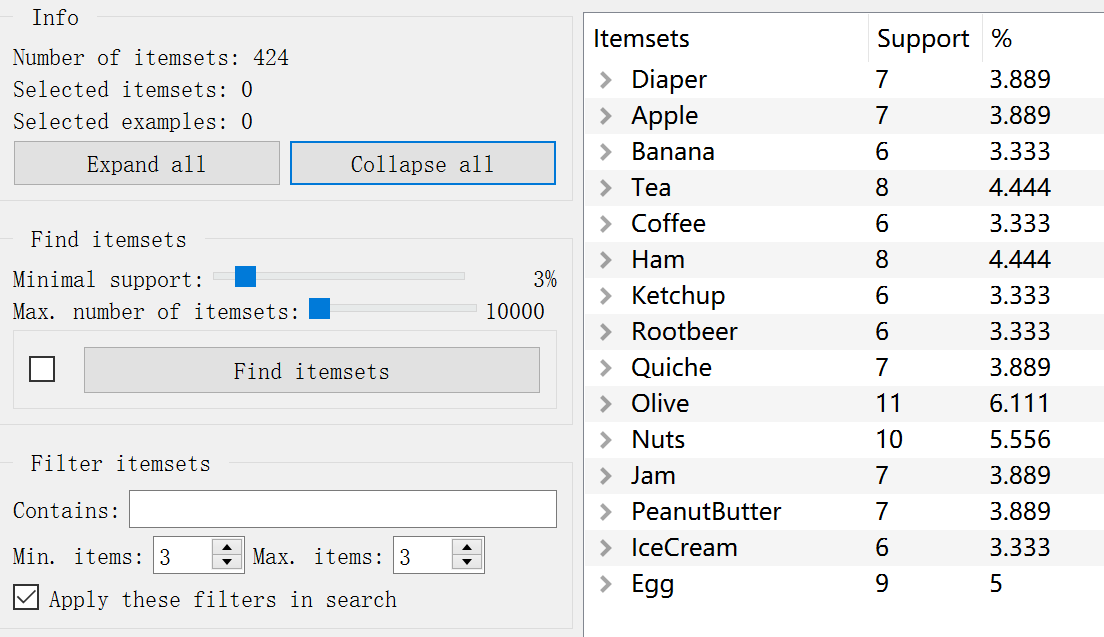
\includegraphics[width=0.49\textwidth]{minsup3_3.PNG}
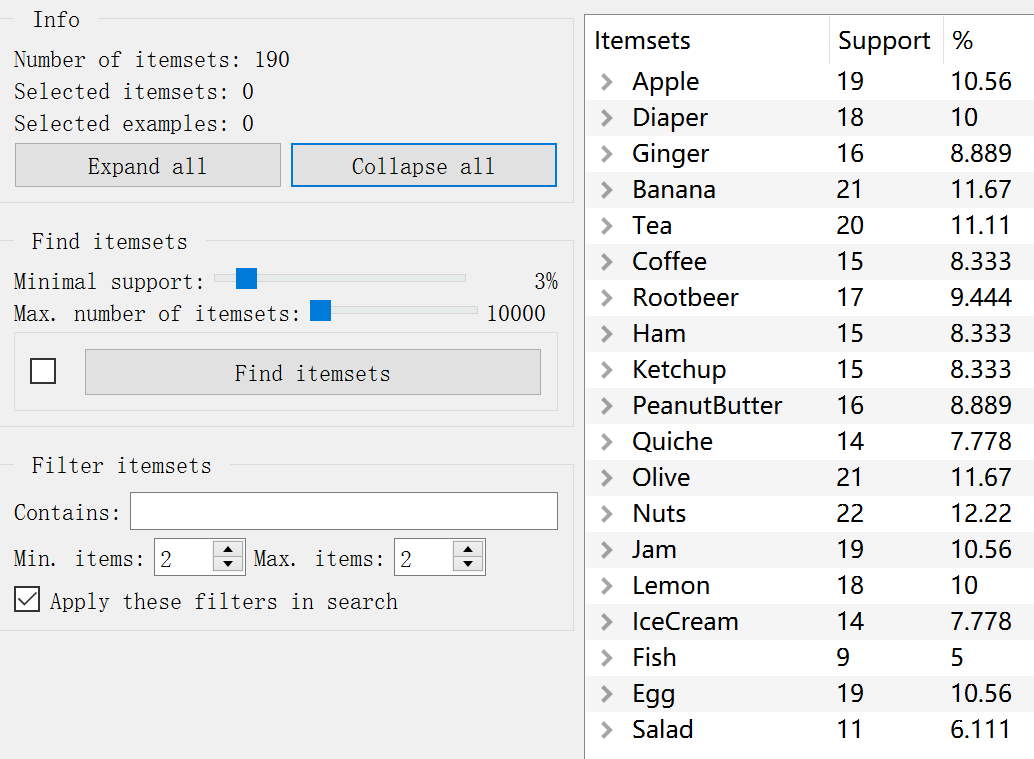
\includegraphics[width=0.49\textwidth]{minsup3_2.PNG}
\end{center}

\begin{center}
\begin{tabular}{rrrr}
\hline
Minimum Support (\%) & No. of Frequent Itemsets & No. of Frequent 3-Itemsets & No. of Frequent 2-Itemsets\\
3 & 659 & 424 & 190\\
\hline
\end{tabular}
\end{center}

Percentage of frequent 3-itemset = 424 / 659 = 64.34\%

Percentage of frequent 2-itemset = 190 / 659 = 28.83\%

\section{Question 3:}
\label{sec:orgb704839}
\begin{center}
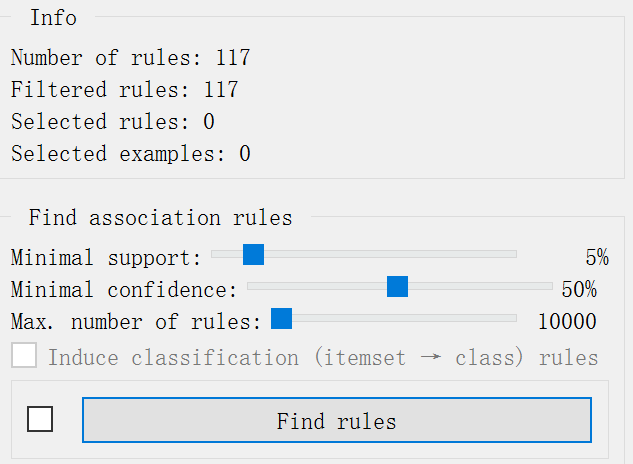
\includegraphics[width=0.49\textwidth]{minsup5_mincon50.PNG}
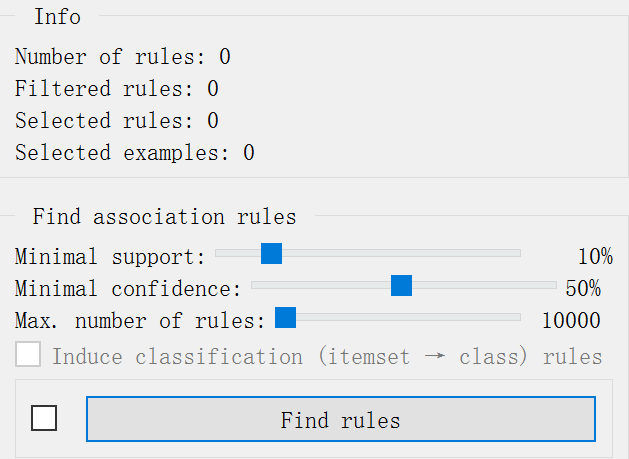
\includegraphics[width=0.49\textwidth]{minsup10_mincon50.PNG}
\end{center}

\begin{center}
\begin{tabular}{rrr}
\hline
Minimum Support (\%) & Minimum Confidence (\%) & No. of Association Rules\\
5 & 50 & 117\\
10 & 50 & 0\\
\hline
\end{tabular}
\end{center}

Explanation: The smaller the minimum support is, the more the number of strong rules generate.

\section{Question 4:}
\label{sec:org278a48c}
\begin{center}
\begin{center}
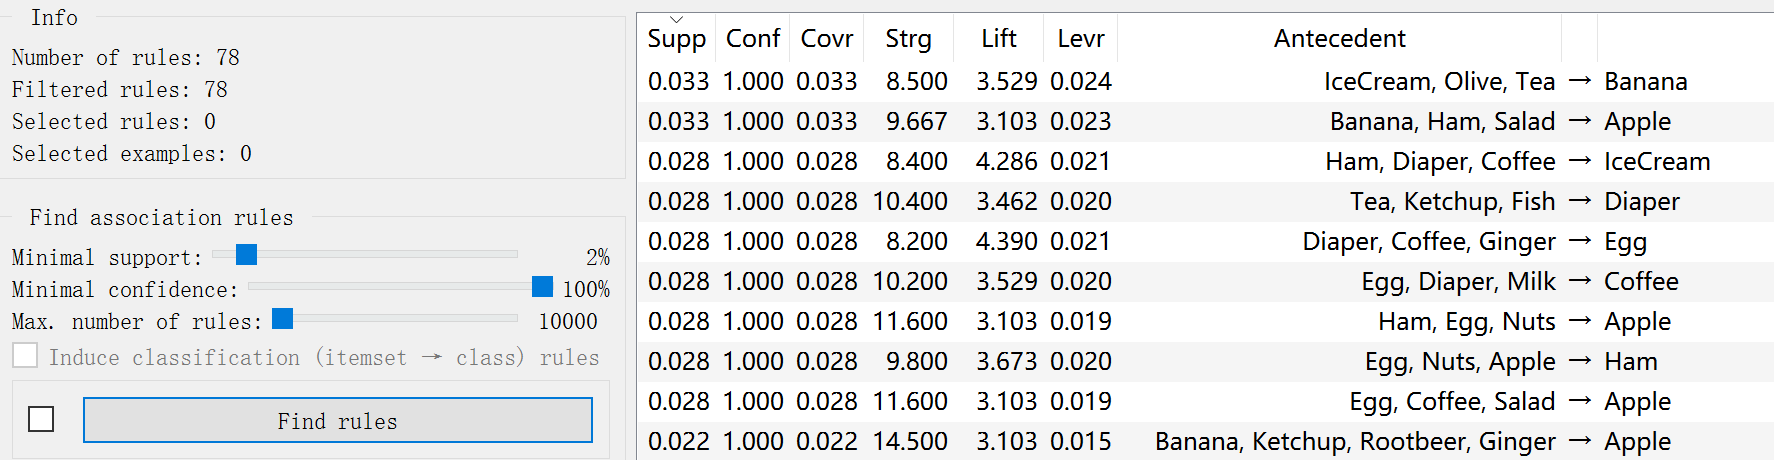
\includegraphics[width=.9\linewidth]{mincon100_3.PNG}
\end{center}
\end{center}

Rule1: Ice Cream, Olive, Tea --> Banana (minsup=3.3\%)

Rule2: Banana, Ham, Salad --> Apple (minsup=3.3\%)

Rule3: Ham, Diaper, Coffee --> Ice Cream (minsup=2.8\%)

\section{Question 5:}
\label{sec:orgc8525df}
\begin{center}
\begin{center}
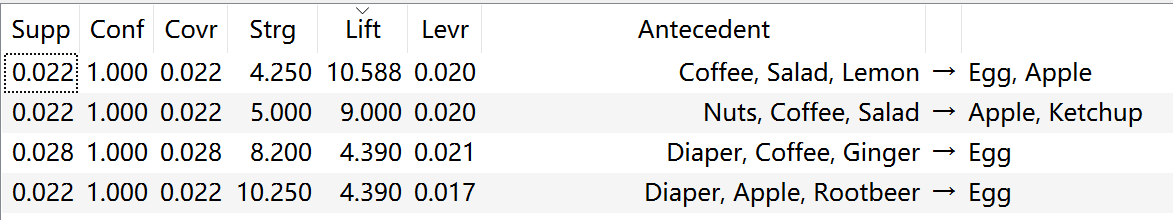
\includegraphics[width=.9\linewidth]{interest.PNG}
\end{center}
\end{center}

Interesting Rules:

Coffee, Salad, Lemon --> Egg, Apple   (Minsup=2\%, Minconf=100\%, Lift = 10.588)

Nuts, Coffee, Salad --> Apple, Ketchup     (Minsup=2\%, Minconf=100\%, Lift = 9)

These are the two most interesting rules I found when minimum support is 2\%
and minimum confidence is 100\%. The measure used to identify the
interestingness of the rule is lift. Lift shows the correlaton between the two
itemsets. If the lift of the rules is high, it means the probability of
occurrence of the antecedent is low. The higher the value of lift is, the more
positively correlated these two datasets are.
\end{document}
